\documentclass{beamer}
\usepackage{amsmath}
\usefonttheme[onlymath]{serif}
\usetheme{Boadilla}
\title[Stable Matching for Dynamic Ride-Sharing ]{Stable Matching for Dynamic Ride-Sharing Systems}
\author[Iain Rudge, Tom Manderson]{Iain Rudge\\Tom Manderson}
\date{31st August, 2017}
\begin{document}
\begin{frame}
	\titlepage
\end{frame}

\begin{frame}
\frametitle{Problem Description}
\begin{itemize}
	\item Vehicles typically have capacity for extra passengers
    \item Presents a cost-saving opportunity for drivers
    \item ``Ride sharing" refers to situations where costs are less for all participants, driver does not make money
    \item Attempting to maximise both system-wide and individual cost saving
\end{itemize}
\end{frame}

\begin{frame}
\frametitle{Stability in Matching}
\begin{columns}
\column{.6\textwidth}
  \begin{itemize}
  \item Maximising system-wide savings does not necessarily result in the best outcome for individuals
  \item Maximising individual preferences is guaranteed to be 
  \item Paper introduces notion of ``stability" and ``price of stability"
  \end{itemize}

\column{.4\textwidth}
  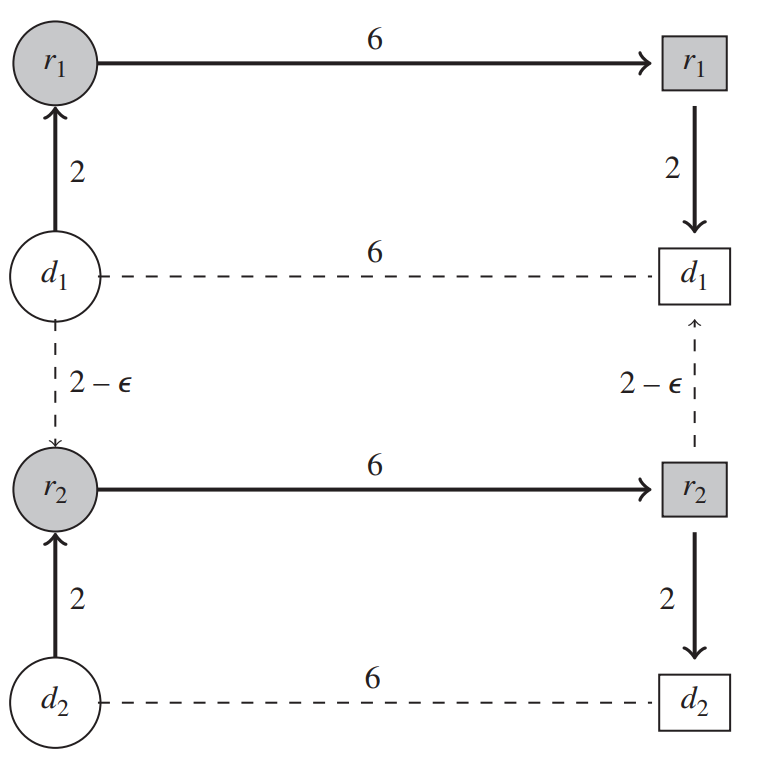
\includegraphics[width=\textwidth]{stability.png}
\end{columns}
\end{frame}

\section{Model}
\begin{frame}
\frametitle{Model Data}
\begin{itemize}
	\item \(P\), set of all locations
	\begin{itemize}
		\item Distance \(D(a, b) \in R\) between any pair \(a, b \in P\) must be known
		\item No other requirements
	\end{itemize}
	\item \(S = D \cup R\), set of all announcements
	\begin{itemize}
		\item \(D\), set of driver announcements
		\item \(R\), set of rider announcements
		\item Comprised of data (as functions of \(s \in S\))
		\begin{itemize}
		 	\item origin \(o(s) \in P\)
		 	\item destination \(d(s) \in P\)
		 	\item earliest departure time \(t_d(s)\in R\)
		 	\item latest arrival time \(t_a(s) \in R\)
		\end{itemize} 
	\end{itemize}
    \item \(A\), set of valid rider-driver matchings: \(\forall (i, j) \in A \cdot i \in R, j \in D\)
\end{itemize}
\end{frame}

\begin{frame}
\frametitle{Model}
Variables
\begin{equation*}
x_{i,j} = \begin{cases}
1 & (i,j) \text{ is used} \\
0 & \text{ otherwise }
\end{cases}
\quad \forall (i,j) \in A
\end{equation*}
\[\]

Constraints
\[\sum_{j \in D} x_{i,j} \leq 1 \quad \forall i \in R\]
\[\sum_{i \in R} x_{i,j} \leq 1 \quad \forall j \in D \]
\[\sum_{j` \geq j_i} x_{i,j`} +  \sum_{i` \geq i_j} x_{i`,j} + x_{ij}\geq 1 \quad \forall (i,j)\in A \]

Objective
\[\max \sum_{(i,j) \in A} x_{i,j}\left(D(o(j), d(j)) - D(o(j), o(i)) - D(d(i), d(j)) \right)\]
\end{frame}

\begin{frame}
\frametitle{Data Generation}
\begin{itemize}
\item Reached out to original paper authors to acquire data used in paper
\begin{itemize}
\item Yet to hear back
\item Investigated original data source, but the dataset is mostly irrelevant
\item Prohibitively time consuming to manipulate data
\end{itemize}
\item Generating our own dataset
\begin{itemize}
\item Locations generated based on uniform randon \(x,y\) pairs
\item Announcements uniformly select distinct origin and destination
\item Start time uniformly selected, end time generated based on travel time and flexibility
\item Quantity of locations and announcements still being tested, totally configurable
\end{itemize}
\end{itemize}
\end{frame}

\begin{frame}
	\frametitle{Proposed Solution}
    \begin{itemize}
    	\item Basic model
    		\begin{itemize}
    			\item Duplicate model used in paper 
                \item Solve using standard Gurobi IP solver 
    		\end{itemize}
		\item Marginal Solution
    		\begin{itemize}
    			\item Implement basic solution in Gurobi IP solver  
                \item Use Lazy constraints to account for preferences
                \item \(M^P\), set of all positive matches
                \item \(M^N\), set of all negative matches
                \item Positive Preference \(x_{ij} = 1 \quad \forall mp \in M^P\)
                \item Negative Preference \(x_{ij} = 0 \quad \forall mn \in M^N\)
				\item Forcing Branches on positive preferences and discarding them on negatives
    		\end{itemize}
    \end{itemize}

\end{frame}

\begin{frame}
	\frametitle{Proposed Solution}
\begin{itemize}
         \item Multiple Riders
         \begin{itemize}
         	\item Potential for delayed column generation, more investigation needed
            \item Three cases present
            \begin{itemize}
            \item Pick up additional riders on route
            \item All riders travel to a start location   
            \item Chaining riders
            \end{itemize}
         \end{itemize}
         
\end{itemize}

\end{frame}
\begin{frame}
	\frametitle{Challenges}
    \begin{itemize}
    	\item Multiple riders
        \begin{itemize}
        	\item Three cases to consider as mentioned prior 
            \item Massive increase to amount of Arcs generated
            \item More complex arc generation required
        \end{itemize}
        \item Arc generation 
        
       \begin{itemize}
       		\item Naive method currently implemented 
            \item More elegant solutions will allow for faster run-time
            \item Potential to solve using an optimization sub-problem
            \item Handling ties to use linear relaxation
       \end{itemize}
    \end{itemize}

\end{frame}
\end{document}